\section{Data-science methods and additional results}\label{app:datascience-results}

This appendix records the population, prediction, selection and search
methods supporting Section~\ref{sec:black-box-datascience}, together with
the additional numerical diagnostics and their interpretation limits.

\subsection{Exact profile of equilateral-triangle products}
\label{app:ds-triangle-profile}

For the family in \eqref{eq:ds-triangle-profile}, the capacity is
\[
 c_{\mathrm{EHZ}}(T_\theta)=\frac{3\sqrt3}{4\cos(\pi/6-d_3)}.
\]
Here is a direct proof in the manuscript's quadratic-program convention.
Choose the outward normals
$n_i=(\cos(2\pi i/3),\sin(2\pi i/3))$, $i=0,1,2$, so
$P_3=\{q:n_i\cdot q\leq1/2\}$, and write
$m_j=\operatorname{Rot}(\theta)n_j$. The six dual rows are
$a_{q_i}=(2n_i,0)$ and $a_{p_j}=(0,2m_j)$.

Closure forces a common weight $x$ on the three $q$ rows and a common
weight $y$ on the three $p$ rows, with $x+y=1/3$. Indeed, the kernel of
the three-normal matrix is spanned by $(1,1,1)$. A positive quadratic
objective requires $x,y>0$, so all six rows occur. For their order,
\[
 Q=4xyS,\qquad
 S=\sum_{i,j}\epsilon_{ij}n_i\cdot m_j,
\]
where $\epsilon_{ij}=1$ if $q_i$ precedes $p_j$ and $-1$ otherwise.
Cyclically moving the first row to the end preserves $S$, since both
normal sums vanish. Classify the cyclic words by their number of $q$
runs, equal to their number of $p$ runs.

With one run, $S=0$. With two runs, the two $q$ block sums are $u,-u$
with $u=\pm n_i$, and the two $p$ sums are $v,-v$ with $v=\pm m_j$.
The reduced word $u,v,-u,-v$ gives $S=2u\cdot v\leq2$. With three
runs the word alternates, say $q_a,p_b,q_c,p_d,q_e,p_f$, and
\[
 S=2\bigl(n_a\cdot m_b+(n_a+n_c)\cdot m_d\bigr)
  =2(n_a\cdot m_b-n_e\cdot m_d).
\]
Set $c_k=\cos(\theta+2\pi k/3)$. On $0\leq\theta\leq\pi/6$ we have
$c_0\geq c_2\geq c_1$, so all words satisfy
\[
 S\leq2(c_0-c_1)=3\cos\theta+\sqrt3\sin\theta.
\]
The bound is at least three, so it covers the two-run case too. Equality
is attained by $q_0,p_0,q_2,p_2,q_1,p_1$. Since $xy\leq1/36$, with
equality at $x=y=1/6$, we obtain
\[
 Q_{\max}=\frac{3\cos\theta+\sqrt3\sin\theta}{9}
         =\frac{2\sqrt3}{9}\cos(\pi/6-\theta).
\]
The capacity formula follows from $c=1/(2Q_{\max})$. As
$\operatorname{area}(P_3)=3\sqrt3/4$ and
$\operatorname{vol}_4(T_\theta)=27/16$, the ratio is
$\tfrac12\sec^2(\pi/6-\theta)$.

All edges have length $\sqrt3$, and their directions differ from the
corresponding normals by a common quarter-turn. The mixed-edge sum is
therefore $9\sum_{k=0}^2|c_k|$. On this sector $c_0\geq0$,
$c_1,c_2\leq0$ and $\sum_k c_k=0$, giving $18\cos\theta$.
Dividing by $3\sqrt3/4$ yields $R=8\sqrt3\cos\theta$.

To reduce other angles, both quantities are even under simultaneous
reflection in the factor planes and have period $2\pi/3$ by triangle
symmetry. The symplectic factor exchange $(q,p)\mapsto(p,-q)$, followed
by rotation through $-\theta$ in both planes, sends $T_\theta$ to
$T_{\pi-\theta}=T_{\pi/3-\theta}$. Together with evenness this gives
period $\pi/3$, proving the formulas with $d_3$. Both expressions
strictly decrease as $d_3$ runs from zero to $\pi/6$.

The connection to covariance balancing is also exact. For a centered
triangle with vertex matrix $X\in\mathbb R^{2\times3}$, isotropic vertex
covariance means $XX^T=3\alpha I_2$, and $X\mathbf1=0$. Hence
\[
 X^TX=3\alpha(I_3-\mathbf1\mathbf1^T/3).
\]
All squared distances between different vertices equal $6\alpha$, so
the triangle is equilateral. Independent factor dilations preserve both
$R$ and $\operatorname{sys}$; thus ideal balancing of two triangles
places their product in the family above. The rounded numerical outputs
are close to this family, not asserted to have exactly equilateral
binary64 coordinates.

\subsection{Sampling and retained data}\label{app:ds-generation}

A polytope was specified by inequalities
\[
 K=\{x:\langle n_i,x\rangle\leq h_i,\quad i=1,\ldots,F\}.
\]
For the generic family, each $n_i$ was independent and uniform on the unit
sphere in $\mathbb R^4$: we normalized a vector of four independent standard
Gaussian coordinates. The heights were independent and uniform on
$[0.8,1.2)$. A proposed body was retained only if it was bounded and every
proposed inequality defined a facet. The construction also rejected zero or
near-duplicate normals. These conditions are part of the sampling law;
``random polytope'' here does not mean a uniform choice from all convex bodies.

The original population contains 512 bodies for each generic facet count
and 1,024 for each product side-count pair. The retained generator records
identify seed 42; product seed/attempt metadata cannot be independently
reconstructed from the recovered cache. The source geometries, row identifiers
and stored numerical values are nevertheless matched for every body.
The reproduction records are listed in Table~\ref{tab:ds-evidence-index}.

\subsection{Numerical evaluation and retrospective checks}\label{app:ds-evaluation}

The complete historical source geometry was recovered and matched to all
14,336 table rows. A geometry-only rebuild restored six later descriptors;
all 645,120 overlapping table cells agreed. This retained the historical
volume normalization and did not evaluate capacity.

A separate current-evaluator run attempted every body. It returned 14,245
successful evaluations, 54 input-policy failures and 37 scalar-tolerance
failures. Among successful rows, the largest relative differences were
$1.06\cdot10^{-14}$ in capacity, $3.14\cdot10^{-14}$ in volume and
$3.23\cdot10^{-14}$ in the ratio. No row is dropped from the original
statistical analysis. The original failures are retained alongside the separate follow-up below.

A subsequent interval-preserving evaluation recovered results for 90 of
those refusals. The 37 scalar-tolerance refusals yielded capacity intervals
without changing their input bodies. Exact power-of-two rescaling brought
53 of the 54 norm-policy failures into the admitted range; fresh geometry
checks preceded evaluation, and homogeneity transferred their interval
endpoints back to the original bodies. Across both runs, 14,289 bodies have
accepted capacity scalars at tolerance $10^{-10}$ and another 46 have wider
capacity intervals. One body, \texttt{random\_F8\_s3\_45}, remains unresolved.
No policy or tolerance was relaxed. The complete sample, including this
body, remains in the historical statistical analysis.

The current evaluator reconstructs the geometry of the stored binary64 input
and returns rational product capacities or outward capacity bounds. Its
volume calculation remains floating-point. Agreement of central values does
not mean that a narrow new interval contains an independently rounded old
value: 5,583 old capacity scalars lie outside the new intervals despite the
small differences above. The initial reevaluation corroborates the numerical values
on its successful bodies; it does not certify the original execution or the
complete ratio. Prospective selection experiments and optimizer traces have
their own evidence records and are not validated by this baseline comparison.

\subsection{Prediction models and feature families}\label{app:ds-prediction}


Prediction experiments gave another view of the signal. A random forest~\cite{dsBreiman2001},
which averages predictions from many decision trees, used 39 descriptors:
27 describing face counts and incidences, and 12 summarizing ridge areas.
The test split held out groups defined by capacity-source label and facet
count, leaving 8,192 training rows and 6,144 test rows. Its test coefficient
of determination was $R^2=0.885$. Here
\[
 R^2=1-\frac{\sum_{i\in\mathrm{test}}(s_i-\widehat s_i)^2}
                   {\sum_{i\in\mathrm{test}}(s_i-\overline s_{\mathrm{test}})^2}
\]
compares squared prediction error with prediction by the test-set mean.
Here $s_i$ is the observed numerical systolic ratio and $\widehat s_i$
is the model prediction.
The mean absolute error was $0.0495$. This was one group split, not repeated
cross-validation across independent datasets.

A separate feature-family comparison used histogram-based gradient-boosted
regression~\cite{dsSklearnHGB}, which successively fits trees to improve the prediction. Under
its common training/test split, ridge-area features alone gave $R^2=0.887$,
whereas combinatorial counts alone gave $0.043$. The comparison points to
information in the ridge areas beyond those counts. Its split and feature
list differ from the random-forest experiment, so the two scores do not rank
the learning algorithms against each other.


\subsection{Selection and comparison rules}\label{app:ds-selection}

The 100,000-product concentration experiment specified a positive aggregate
mean difference and positive differences in at least seven of ten groups
as its continuation criterion. It found eight positive groups and a mean
difference of about $0.034$. This is the descriptive design criterion;
no significance claim is attached to passing it.

For the tangential-generator comparison, controls were selected by a fixed
hash order, before capacity evaluation, from the eligible pool after removing
the union of the ridge and covariance selections. They are unselected
same-generator comparisons, not an asserted random sample of the full pool.

The opposing $3\times6$ and $4\times4$ rotation paths contain four recorded
positions each. Their simultaneous decrease in ridge score and numerical
ratio is a finite observation; monotonicity at every intermediate angle
was not established.

\paragraph{Initial ridge selection.}
The preliminary pool contained 100,000 products. Thirty scalar selection
sets and their baselines required 1,675 distinct evaluations; their union
had maximum recorded ratio $0.868$. The low-$R$ rule selecting ten bodies
per side-count group gave mean $0.6261166821$, against $0.3155039434$ for
ten comparison bodies from each group. Comparison bodies were selected by
a rule-specific fixed hash order excluding the selected set. Overlapping
rules are not independent repetitions.

\paragraph{Restriction to the low-ridge tail.}
The conditional comparison uses 1,000 evaluated products from the lowest
one percent by $R$, with 100 in each side-count group. Spearman
correlations within groups range from $-0.315$ to $+0.301$; pooling ranks
computed separately within each group gives $+0.03197$. Selecting the
most extreme tenth increases the mean in only two of ten groups. The
broad and conditional panels are different generated samples, so their
comparison concerns a change in population and score range. The retained
analysis is in \path{tail-dependence-feasibility/artifacts/current/},
under the methods directory in Table~\ref{tab:ds-evidence-index}.

\paragraph{Conditioning the original dataset.}
A separate analysis retains the lowest-$R$ or highest-ratio fraction within
each of the eighteen original sample groups. At retained fractions
$100\%,20\%,10\%,5\%,1\%$, both arms contain respectively
14,336, 2,874, 1,446, 728 and 158 bodies. There are no ties across these
cutoffs. Each retained group is reranked independently; its two rank
columns are divided by the group's retained size, then pooled for a
Spearman correlation. Thus the summary weights bodies rather than giving
each group equal weight. The low-$R$ values are
$-0.944,-0.434,-0.222,-0.113,+0.035$, and the high-ratio values are
$-0.944,-0.496,-0.286,-0.239,-0.036$. The smallest panels contain only
six generic or eleven product bodies per group. These are descriptive
statistics under conditioning, not evidence of independence, systematic
reversal, or the effect of a shape intervention. Row identities, cutoffs
and a second rank calculation were independently checked; the reproducible
packet is \path{experiments/sys-datascience/methods/selection-mechanism/}.

\paragraph{Gaussian rank reference.}
Each original sample group is assigned a bivariate Gaussian reference
with Pearson correlation $2\sin(\pi r_s/6)$, where $r_s$ is its observed
full-sample Spearman correlation. One thousand simulations preserve all
eighteen group sizes and apply the same conditional ranking statistic.
At the five-percent cutoff, the reference means are $-0.695$ for both
selection directions. The central simulation intervals are
$[-0.738,-0.649]$ for high-ratio selection and $[-0.736,-0.647]$ for
low-$R$ selection, against observed values $-0.239$ and $-0.113$.
These are pointwise simulation references with fitted parameters held
fixed. The model was considered after seeing the attenuation; this is
not a prespecified model test or a confidence interval for the observed
correlation. The reference, reproducible simulation and input hashes are
in the same packet's \path{gaussian-result.md} and
\path{gaussian-artifacts/}.

\paragraph{Covariance selection.}
Two fresh pools of 50,000 candidates compared the lowest $0.5\%$ by
$\rho$, the lowest $1\%$ by $R$ followed by its lower half by $C$, and
25 comparison bodies per side-count group. An ordinary covariance
conditioning cutoff excluded three candidates across the two pools.
Controls were selected by fixed hash order from the eligible bodies after
removing both geometric selections. There were 500 memberships in each
selection and 1,436 distinct evaluations. All twenty covariance-minus-
control group effects were positive, ranging from $0.259639$ to $0.440029$.
The mean effect was $0.333123$, while the mean covariance-minus-ridge
effect was $0.014488$; thirteen of the latter twenty effects were positive.

The retained analysis also gives nominal Student-$t$ intervals. They are
$[0.310,0.356]$ for covariance versus controls and $[-0.0149,0.0439]$
for covariance versus ridge selection, using the twenty group effects
and nineteen degrees of freedom. The groups have fixed, different side
counts, and no common-mean sampling model or calibrated coverage for
repeating the complete selection procedure was established. The main text
therefore reports the observed consistency across groups.

\paragraph{Generic and tangential transfer.}
The generic ten-facet experiment selected 100 of 10,000 bodies by lowest
mean normalized ridge area, with 100 disjoint, deterministically selected
comparison bodies. The mean contrast was $0.287$, with a percentile
interval $[0.250,0.324]$ from 20,000 resamples. The ten most extreme
scores minus the other ninety had mean contrast $-0.0318$ and interval
$[-0.0946,0.0331]$. These resamples hold the selected panels fixed; they
do not regenerate the pool, rerank its bodies or reselect its tail.
The selected-panel rank correlation between mean ridge area and ratio
was $+0.149$.

The tangential-source comparison required both original and changed
factors to be admissible and normalized the changed factors separately to
area one. One pool supplied 3,200 eligible bodies in each of the
$4\times6$ and $6\times6$ groups. Each selection had sixteen memberships
per group. Five overlapping selections gave 91 distinct evaluations.
The equally weighted group effects were $0.259$ for covariance versus
controls and $0.225$ for ridge versus controls; their within-panel
resampling intervals were $[0.192,0.329]$ and $[0.160,0.296]$.
These condition on the observed panels. Shared controls make the two
comparisons dependent.

\paragraph{Euclidean area and alignment.}
For the generic selected and comparison panels, the respective means of
$\overline E$ are $0.9167$ and $1.3653$, and the means of
$\overline\kappa_E$ are $0.3769$ and $0.5029$. Within the selected
panel, the ten lowest $R/N_2$ values have mean $\overline E=0.9419$
and mean $\overline\kappa_E=0.3400$, compared with $0.9139$ and
$0.3810$ for the other ninety bodies. These are means of body-level
quantities; they do not assert a factorization of the population mean
of $R/N_2$. Definitions, per-ridge values and the decomposition check
are retained in
\path{experiments/sys-datascience/methods/ridge-tail-anatomy/}.

\subsection{Paired height changes and ambient rotations}
\label{app:ds-deformations}

The paired support-height experiment used sixteen independently generated
pairs of polygons, eight $4\times4$ and eight $4\times6$. For each,
the original product was compared with equalizing heights in the first
factor, the second, or both; all four constructions had to be valid before
any ratio was evaluated. Each factor was scaled to area one. All 64
evaluations succeeded. Changing both factors improved eleven pairs and
worsened five, with mean numerical change $0.0153$. The group means were
$0.0040$ and $0.0266$ respectively. This is the jointly admissible source,
not an unconditioned statement about all polygon pairs.

Recomputing $R$ from the retained paired geometries gives opposite signs
of $\Delta R$ and $\Delta\widehat{\operatorname{sys}}$ in fifteen of
sixteen both-factor changes. The one exception has $R$ increasing from
$11.074$ to $11.218$ while the numerical ratio increases from $0.419$
to $0.436$. The one-factor comparisons have opposite signs in thirteen
and fourteen of sixteen pairs. All 64 bodies have $R\geq11.065$ and
numerical ratio at most $0.742$. These results reuse the retained capacity
evaluations; no new capacity calls enter the comparison. Reconstruction,
row identity and hash checks are recorded in
\path{experiments/sys-datascience/methods/selection-mechanism/controlled-result.md}.

For ambient rotations, the action is
\[
 P\times Q\longmapsto U(P\times Q),\qquad U\in SO(4).
\]
It preserves Euclidean shape and volume. A nonsymplectic $U$ can change
capacity, and the image need no longer be a Lagrangian product for the
fixed symplectic form. One allocation evaluated a source product, a
symplectic rotation control and fourteen prescribed orthogonal rotations;
the other evaluated sixteen fresh products, sharing the source body.
There were four comparisons, two each for $3\times3$ and $4\times4$.
The schedule used fourteen fixed matrices, not uniform sampling over
$SO(4)$. The shared starts gave 124 distinct requests and 128 memberships;
symplectic controls preserved numerical ratios within $4\cdot10^{-16}$.

Rotation improved three starts, but fresh sampling attained a larger
maximum in all four comparisons. In one quadrilateral example, rotation
raised $0.328$ to $0.529$, while fresh sampling reached $0.774$.
Rotation evaluations also took longer. These are observations about the
prescribed schedules and starts, not a comparison of all ambient rotations
with all products from the source law.

\subsection{Factor covariance balancing}\label{app:ds-balance}

The paired comparison uses 32 original products from each of the ten
side-count groups. The selection is fixed by hashes of row identifiers,
without using the target ratios. For planar vertex covariances $A,B$, the
maps $(\det A)^{1/4}A^{-1/2}$ and $(\det B)^{1/4}B^{-1/2}$ have determinant
one and make each covariance scalar. There is one original and one
transformed body for every selected row, evaluated through the same
current product-capacity route. All 640 evaluations succeeded.

The mean numerical ratio changes from $0.341888$ to $0.653683$; 314
paired changes are positive and six are negative. The mean $R$ changes
from $23.738833$ to $11.652347$, with 306 decreases and fourteen
increases. The pooled within-group rank correlation changes from
$-0.928922$ to $-0.248680$. The balanced triangle-product group has
correlation $+1$; the other nine groups range from $-0.571$ to $-0.098$.
Thus the pooled weakening does not mean that every transformed group has
negligible or negative dependence.

The transformed covariance ratios differ from one by at most
$5.1\cdot10^{-13}$, and relative factor-area changes are below
$3.2\cdot10^{-13}$. The original current evaluations agree with their
retained historical numerical ratios within $1.3\cdot10^{-15}$.
These are paired transformations of retained source bodies, not a new
independent population or a test isolating the scalar $\rho$ from other
changed geometric properties. The producer, frozen inputs, evaluator
identity and complete paired results are retained in
\path{experiments/sys-datascience/methods/selection-mechanism/balance-artifacts/}.

\subsection{Finite-budget local optimizer comparison}
\label{app:ds-local-optimization}

The run configuration labels the \(64\) starting bodies as held out.
The saved hashes identify the seven configurations used, but do not establish
that these bodies were absent from earlier development or tuning. A later
development configuration reuses \(16\) starts. Their earlier selection history
is therefore unresolved; this does not show that the reported outcomes were
used to select the configurations.

Every run used the same allocation rule: a nominal \(1000\)\,ms
start-new-work cutoff for charged full-evaluator plus optimizer time and a cap
of \(128\) full historical-evaluator calls.  In-progress work could complete
atomically past the cutoff, and methods could terminate early, so realized
compute differs across runs.  The \(448\) traces contain \(28824\) full calls.
Using the historical numerical objective described in
Section~\ref{subsec:black-box-datascience-finite-budget-optimization},
four-anchor branch history has the largest comparison-block median best value,
\(0.9848\), followed by transition prediction at \(0.9816\) and the finite-gap
affine model at \(0.9772\).  No run reaches
a recorded numerical ratio of one.

\paragraph{The implemented optimizer steps.}
Except for the literal gradient, the methods remove the fifteen infinitesimal
symmetry directions from the forty dual-normal coordinates. The local models
and coordinate poll recompute this transverse space at their anchors;
CMA-ES keeps its initial space. The literal gradient uses the ambient
coordinates.  Every
outer proposal is checked by a fresh geometry reconstruction and the
configured full orbit-word search.  The implementations below are frozen
comparison points; their parameters are not claimed to optimize the
corresponding algorithm families.

\begingroup
\small
\begin{longtable}{@{}>{\raggedright\arraybackslash}p{0.24\linewidth}p{0.67\linewidth}@{}}
\caption{One outer iteration of each optimizer in the recorded
comparison.}
\label{tab:black-box-datascience-f10-optimizer-steps}\\
\toprule
method & implemented step\\
\midrule
\endfirsthead
\toprule
method & implemented step\\
\midrule
\endhead
literal and safeguarded branch gradients
& Differentiate one currently minimizing branch.  The literal method takes
  \(a^+=a+0.01D_as_\sigma(a)\) even after a decrease.  The safeguarded method
  projects and normalizes this gradient, accepts only a fully evaluated
  improvement, and expands or halves its distance after acceptance or
  rejection.\\
finite-gap affine model
& Keep the current branch gaps in a \(10\%\) action window, linearize their
  values, and maximize the minimum affine value on a local ball.  Fully
  evaluate the proposal and use the same expand-or-halve distance rule.\\
four-anchor branch history
& Union candidate words from the four most recent full searches, using a
  \(30\%\) action window and normalized beta allowance \(0.3\).  At a nearby
  point, re-solve the named KKT branches, discard transition-infeasible and
  beta-inadmissible solutions, linearize the remaining values, and maximize
  their affine minimum.  Take at most two internal moves before the next full
  evaluation.\\
history with transition prediction
& Use the preceding method, but for a normalized internal move of length at
  least \(0.08\), also predict newly feasible transitions in the move
  direction and evaluate the words thereby generated.\\
CMA-ES
& Fully evaluate a population of eight Gaussian perturbations, then update
  the mean, covariance, and normalized scale from their ranking.\\
coordinate direct search
& Poll both signs of the \(25\) transverse basis axes.  Move to the best
  improvement and double the radius, or halve the radius if no poll point
  improves.\\
\bottomrule
\end{longtable}
\endgroup

The beta allowance applies when retaining candidate words at a discovery
anchor: a raw KKT solution is kept only if
\[
 \frac{\min_i\beta_i}{\max_i|\beta_i|}\geq-0.3
\]
as well as satisfying the action-window cutoff. This retains some words
whose weights are negative at that anchor, in case they become feasible
nearby. It does not relax orbit feasibility: each local model and target
evaluation again checks the word's transitions and the usual nonnegative
weight condition at the point being evaluated.

The two history methods accept any usable outer evaluation, including a
decrease; their reported best-so-far value therefore differs from their
current iterate. The safeguarded gradient and finite-gap method accept only
improvements, multiplying the relative step length by $1.25$ on success
and by $0.5$ on failure. The history methods use up to two internal model
steps between full evaluations.

The companion endpoint packet does not test local maximality.  Signed polls
along the transverse basis find an improving direction at seven of \(16\)
one-second branch-history endpoints and two of the corresponding five-second
endpoints.  Separate validated continuation paths show that even an endpoint
with no improving basis direction can retain appreciable ascent between the
tested axes.  These observations diagnose insufficient finite budgets; they
do not estimate the distance to a local maximum.

\paragraph{Detailed HKO calibration.}
Distances here use the Euclidean norm of the forty ordered dual-row
coordinates $a$, with no further minimization over symmetries. Thus distance
to HKO is $\|a-a_{\mathrm{HKO}}\|_2$, and the fraction removed is
$1-\|a_{\mathrm{after}}-a_{\mathrm{HKO}}\|_2/
\|a_{\mathrm{before}}-a_{\mathrm{HKO}}\|_2$.
The four unit directions lie in the transverse space at HKO: two random
directions, its first chosen basis vector (the slice-basis sentinel), and
the projected, normalized tangent from rotating the pentagon's second
factor (the pentagon-tangent sentinel). The source distances in the figure
are absolute Euclidean distances along these rays.

On \(16\) known perturbations along four development directions from HKO, the
multi-branch continuation accepted no move at HKO and improved every
perturbation.  One step recovered \(93.4\%\)--\(100\%\) of the known evaluator
gap and removed \(77.9\%\)--\(100\%\) of the distance to HKO.  In contrast,
the gradient of one current minimizing branch recovered
\(-22.1\%\)--\(41.4\%\) of the gap.

\begin{figure}[!htbp]
\centering
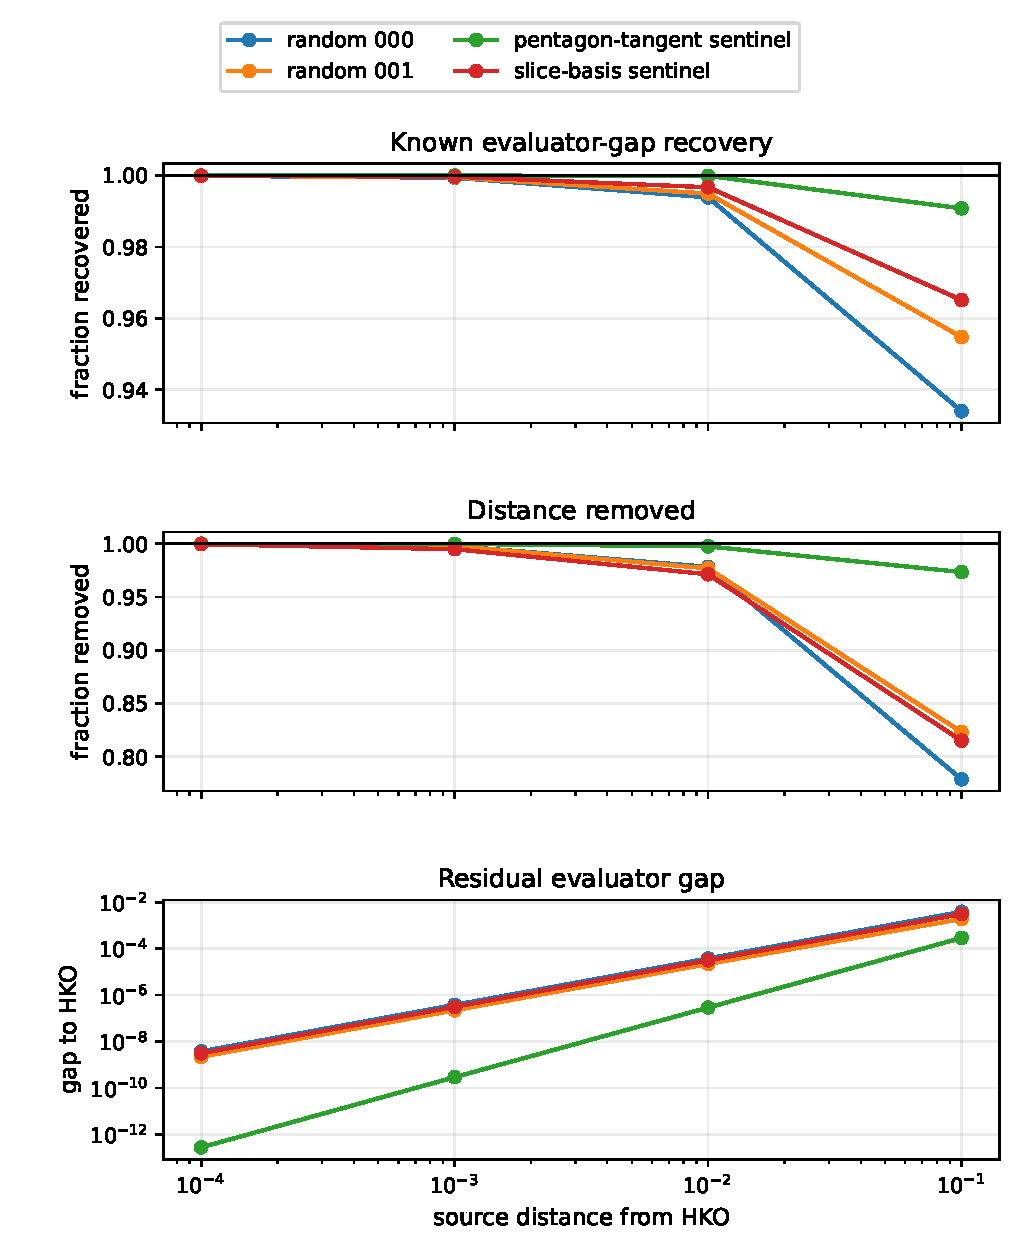
\includegraphics[width=\linewidth]
  {figures/hko-recovery-by-source-distance.pdf}
\caption{One-step calibration on known perturbations of HKO.  From top to
bottom, the panels show recovered evaluator gap, removed distance, and
residual evaluator gap.}
\label{fig:black-box-datascience-hko-optimizer-calibration}
\end{figure}

\paragraph{Selected finite-step failure audit.}
For the following probes and audits, a relative or normalized radius $r$
instead scales a unit direction $u$ by the current state norm:
$\delta a=r\|a\|_2u$. The normalized length of a continuation path is
$\sum_k\|a_{k+1}-a_k\|_2/\|a_k\|_2$.

At the eight highest four-anchor tuning endpoints, five admitted one validated
improvement, by \(1.57\cdot10^{-6}\) to \(4.61\cdot10^{-5}\).  Across the
\(80\) multi-branch proposals, \(52\) decreased the recomputed evaluator value
despite a represented target winner and positive affine prediction; \(40\) of
these losses retained determinate, unchanged geometry.  All \(40\)
current-branch gradient proposals decreased.

The three-proposal audit compared two such failures with one positive control.
At normalized radius \(10^{-5}\), the failures perturbed their named KKT
matrices by \(218\) and \(67\) times the smallest base eigenvalue magnitude
and crossed zero; the control had ratio \(1.53\), did not cross zero, and kept
the correct sign.  At the smallest tested radius, \(10^{-8}\), central
differences approximated the implemented analytic derivatives with relative
errors below \(1\%\) for the named action and \(1.9\%\) for the named branch
ratio.  Binary64 and exact-arithmetic geometry
reconstruction agreed at all \(39\) audited points, and relative volume
discrepancies were below \(10^{-15}\).  For these selected cases the observed
failure is finite-distance nonlinearity of an ill-conditioned KKT branch.

\begin{figure}[htbp]
\centering
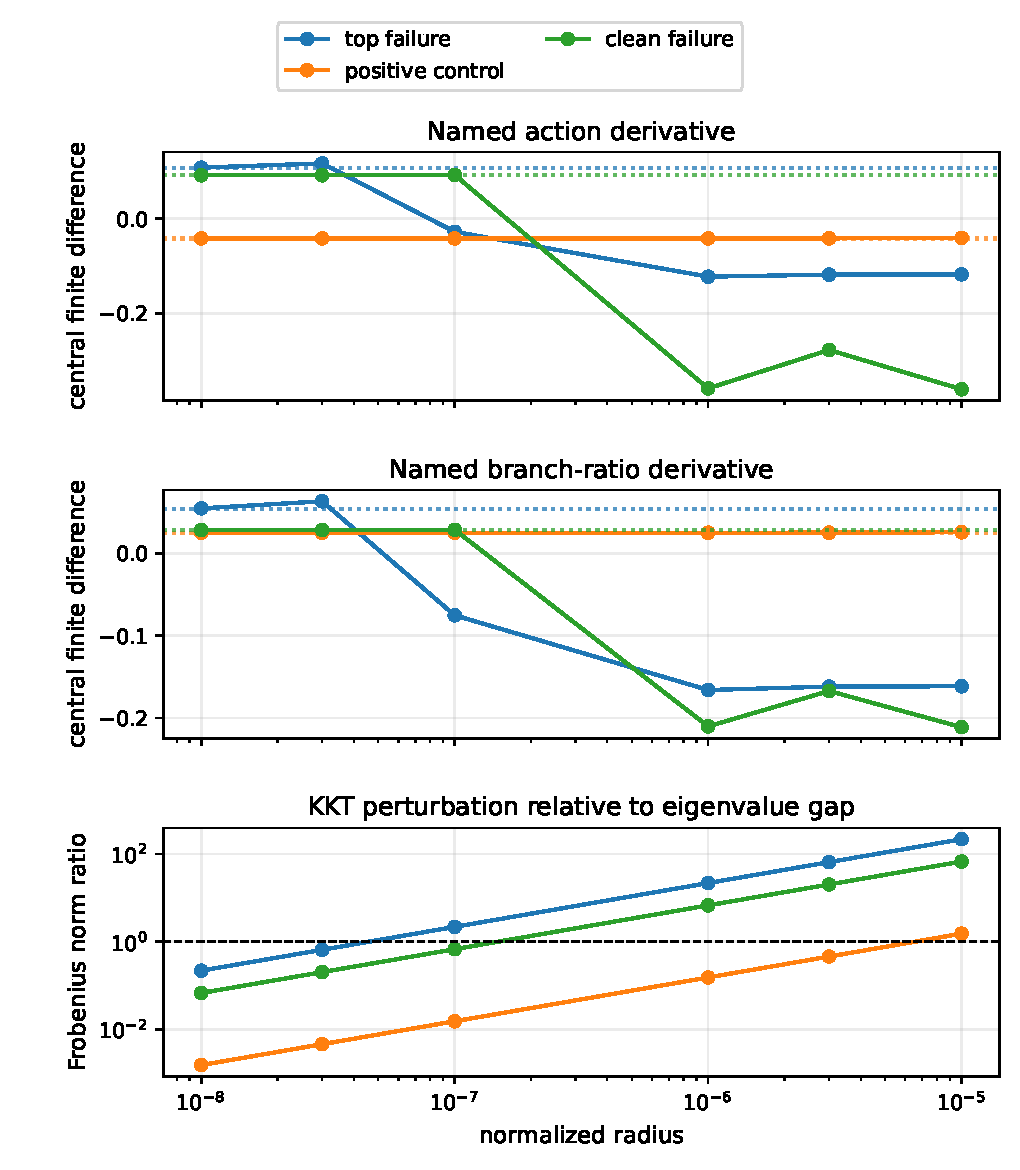
\includegraphics[width=\linewidth]
  {figures/derivative-and-kkt-scale.pdf}
\caption{Finite differences for two failed affine proposals and one positive
control.  Prediction changes regime when the KKT perturbation becomes large
relative to the smallest source eigenvalue magnitude (bottom).  Dotted lines
in the top two panels are the analytic derivatives.}
\label{fig:black-box-datascience-kkt-trust-scale}
\end{figure}

These diagnostics use selected controls rather than population samples.  They
do not provide a convergence theorem, a population error rate, or a universal
conditioning cutoff.

\subsection{Endpoint probes and continuation}\label{app:ds-probes}

Sixteen history-method endpoints were chosen across the observed terminal
performance range. Each received both signs of 25 transverse basis
directions at relative radii $10^{-3}$, $10^{-4}$ and $10^{-5}$, giving
150 probes per endpoint. Seven endpoints had a raw positive change and
nine had none. Rank-based endpoint selection prevents interpreting these
fractions as a population convergence probability.

After a larger budget on those starts, continuation examined three
selected endpoints and HKO. It tested branch-model and selected-gradient
proposals at five decreasing step lengths, with fallback signed basis
polling, and allowed ten accepted improvements. All three endpoints took
ten improving steps; HKO took none. One endpoint with no improving signed
basis direction gained $0.00223$ along oblique moves of total normalized
path length $0.01$.

The separate triangle--hexagon, square--square, CH2021 and pentagon-control
suite used basis, projected random and prescribed rotation directions at
three radii. All 1,482 probes were valid. The three targets had no nominal
gain above $10^{-12}$; the pentagon control had twelve, all from rotations.
Incomplete historical source provenance and broad capacity-derived bounds
prevent interpreting the nominal misses as certified local maximality.

\FloatBarrier
\subsection{Adaptive product sampling}\label{app:ds-adaptive}

Both arms began with the same 64 independently generated products. Four
populations including initialization gave 256 charged evaluations per arm.
The adaptive update used the sixteen bodies with largest ratios. Across
three runs, shared initial populations gave 1,344 actual evaluations and
1,536 arm memberships; all actual evaluations succeeded and all recorded
ratios were below one. The top-eight statistic removes repeated exact
dual-vertex arrays, retaining different arrays with equal scores.

For reproducibility, let $g_1,\ldots,g_5>0$ be the cyclic normal-angle gaps
of a factor and let $r_i$ be its dual-normal lengths. Set
\[
 \ell_i=\log(g_i/g_5)\quad(i=1,\ldots,4),\qquad
 z_i=\log r_i-\frac15\sum_{j=1}^5\log r_j.
\]
We store the first four $z_i$ and recover $z_5=-\sum_{i=1}^4z_i$.
Reconstruction uses
\[
 g_i=\frac{2\pi e^{\ell_i}}{1+\sum_{j=1}^4e^{\ell_j}},\qquad
 g_5=\frac{2\pi}{1+\sum_{j=1}^4e^{\ell_j}},\qquad h_i=e^{-z_i}.
\]
The first normal angle is zero in the first factor and $\phi$ in the second.
The initial IID encoding chooses a cyclic origin by lexicographically
minimizing the sequence of gap/length pairs. Sampled adaptive coordinates
are retained for the updates without another cyclic relabelling.

For an ordinary coordinate $j$, write $\widehat\mu_{E,j}$ and
$\widehat v_{E,j}$ for the mean and population variance of the sixteen elites.
The update is
\[
 \mu_j^+=\tfrac12\mu_j+\tfrac12\widehat\mu_{E,j},\qquad
 v_j^+=\max\{\tfrac12v_j+\tfrac12\widehat v_{E,j},\;0.05v_{0,j}\}.
\]
Initialization uses the population moments of the shared 64 bodies.
Coordinates are drawn independently with these Gaussian moments. The phase
uses circular means, a unit-vector blend of old and elite means, and variance
of angular deviations wrapped into $[-\pi,\pi)$. Samples are wrapped modulo
$2\pi$. A vanishing resultant retains the previous mean; initial fallback
uses the smallest-ID candidate's phase. Ties in elite selection are broken
by candidate ID.

Each population permits at most 640 construction attempts for 64 accepted
bodies. Failed geometry and unsupported evaluator inputs are rejected before
target evaluation; an incomplete population does not trigger an update.
The evaluator admission includes finite, nonredundant bounded geometry and
primal and dual infinity-norm bounds between $10^{-3}$ and $10^3$.
The three seeds are 202609140301, 202609140302 and 202609140303. The retained
report records the stopped first version and the subsequent supported
version separately.

The source restriction needs particular care. An initial version stopped
when one body exceeded the evaluator's admitted primal-vertex infinity-norm range.
The completed version applied the evaluator's existing admission conditions
to both proposal arms before accepting a body for evaluation. This was a
procedural revision after seeing the failure. Both arms reject unsupported
inputs, but the admission test acts on the actual coordinate representation:
IID bodies retain their original representation and adaptive bodies use the
normalized reconstruction. It is not a symmetry-invariant condition on all
pentagon products. The result is therefore for this implemented,
admission-conditioned comparison.

The complete run took $215.8$ seconds: $182.2$ seconds for construction and
admission checks, $32.9$ seconds in evaluator processes, and $0.053$ seconds
for distribution updates. Including construction and charging initialization
to each arm, the adaptive runs used about $35$--$36$ seconds per seed and IID
about $46$--$51$ seconds. Equal evaluation counts did not imply equal cost.
These measured costs favor the adaptive arm in this run; they are not the
outcome of a separate equal-wall-time experiment.


\subsection{Evidence and reproduction index}

Paths in Table~\ref{tab:ds-evidence-index} are relative to the accompanying
repository. Each packet identifies its inputs and analysis; the original
historical optimizer executable and full proposal traces were not recovered.

\begin{longtable}{@{}>{\raggedright\arraybackslash}p{.24\linewidth}>{\raggedright\arraybackslash}p{.70\linewidth}@{}}
\caption{Source packets for the chapter.}\label{tab:ds-evidence-index}\\
\toprule Result & Repository source \\\midrule
\endfirsthead
\toprule Result & Repository source \\\midrule
\endhead
Historical population and replay & \path{docs/ds-evidence-closure/README.md}; \path{experiments/polytope-datasets/retained-lineage.md}\\
Restored features and reevaluation & \path{docs/ds-retrospective-revalidation/geometry-full/README.md}; \path{docs/ds-retrospective-revalidation/target-full/README.md}; \path{docs/ds-retrospective-revalidation/repair/README.md}\\
Feature models & \path{experiments/sys-datascience/methods/prediction-ranking/}; \path{experiments/sys-datascience/methods/standard-baseline-p2/}\\
Fresh selection & \path{experiments/sys-datascience/methods/extreme-scalar-rejection-proposer/}; \path{experiments/sys-datascience/methods/extreme-scalar-rejection-proposer/artifacts/covariance-rho-frozen-validation/}\\
Transfer & \path{experiments/sys-datascience/methods/alternative-source-transfer/}; \path{experiments/sys-datascience/methods/generic-ridge-tail-stage1-target/}\\
Paired support heights & \path{experiments/sys-datascience/methods/paired-tangentialization/}\\
Orientation allocation & \path{experiments/sys-datascience/methods/orientation-allocation/}\\
Adaptive product sampling & \path{experiments/sys-datascience/methods/diagonal-cem-pilot/}\\
Local optimization and diagnostics & \path{experiments/dev-gradient-ascent/optimizer-comparison/}; \path{docs/ds-evidence-closure/search-account.md}\\
Conditional and controlled ridge analyses & \path{experiments/sys-datascience/methods/selection-mechanism/}\\
Conditional ridge correlations & \path{experiments/sys-datascience/methods/tail-dependence-feasibility/}\\
Product ridge geometry & \path{docs/ds-evidence-closure/ridge-mathematics.md};
\path{docs/ds-evidence-closure/triangle-profile.md}; \path{experiments/sys-datascience/methods/ridge-endpoint-path/}\\
\bottomrule
\end{longtable}
